\documentclass[11pt,a4paper]{article}
\usepackage[utf8]{inputenc}
\usepackage[T1]{fontenc}
\usepackage{amsmath,amssymb,geometry,xcolor,lmodern,tikz}
\geometry{margin=1.8cm}
\setlength{\parindent}{0pt}
\setlength{\parskip}{5pt}
\pagestyle{empty}
\usetikzlibrary{calc}
\definecolor{jac}{HTML}{0081a7}
\definecolor{dev}{HTML}{f07167}

\begin{document}

{\Large\bfseries Cartesian path constraint (Jacobian cost)}\\[2pt]
{\small FL controller, two large-amplitude movements --- \texttt{Final\_Code/path\_constraint\_jacobian.py}}

\vspace{4pt}
\fcolorbox{gray}{gray!6}{\parbox{0.97\linewidth}{\textbf{Idea.} We want the hand to stay on the
straight segment from the start $p_0$ to the target $p_f$. LQG can only penalise
\emph{quadratic} functions of the state, but the hand position is a \emph{nonlinear} function of
the joint angles. So we measure how far the hand is \emph{sideways} from the line, linearise that
distance around postures lying on the line, and add its square to the cost at every time step.}}

\begin{minipage}[t]{0.60\linewidth}
\textbf{1. What is penalised: the sideways distance.}
With the forward kinematics $p(\theta)$ ($l_1=30$, $l_2=33$\,cm), the unit direction $a$ of the
line and its unit normal $n$:
\[
a=\frac{p_f-p_0}{\|p_f-p_0\|},\qquad n=\begin{bmatrix}-a_y\\ a_x\end{bmatrix},\qquad
\boxed{\,d(\theta)=n^\top\big(p(\theta)-p_0\big)\,}
\]
$d$ is the signed distance (cm) from the hand to the line: $d=0$ on the line. Motion
\emph{along} the line is free; reaching the target is left to the usual terminal cost.
\end{minipage}\hfill
\begin{minipage}[t]{0.37\linewidth}
\vspace{2pt}
\centering
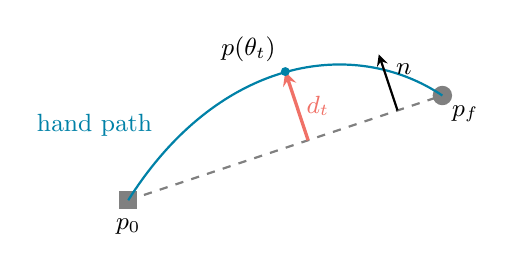
\begin{tikzpicture}[scale=0.95,>=stealth]
  \draw[gray, dashed, thick] (0,0) -- (4.2,1.4);
  \fill[gray] (-0.12,-0.12) rectangle (0.12,0.12);
  \fill[gray] (4.2,1.4) circle (0.13);
  \node[below] at (0,-0.12) {\small $p_0$};
  \node[below right] at (4.2,1.4) {\small $p_f$};
  \draw[jac, thick] (0,0) .. controls (1.2,1.9) and (3.0,2.2) .. (4.2,1.4);
  \coordinate (h) at (2.1,1.72);
  \coordinate (f) at ($(0,0)!(h)!(4.2,1.4)$);
  \draw[dev, very thick, ->] (f) -- (h);
  \fill[jac] (h) circle (0.06);
  \node[above left] at (h) {\small $p(\theta_t)$};
  \node[dev, right] at ($(f)!0.5!(h)$) {\small $d_t$};
  \draw[->, thick] (3.6,1.2) -- ++(-0.25,0.75);
  \node[right] at (3.45,1.75) {\small $n$};
  \node[jac, left] at (0.45,1.0) {\small hand path};
\end{tikzpicture}
\end{minipage}

\textbf{2. Make it linear: use the Jacobian.} $d(\theta)$ is not quadratic in $\theta$. Pick, for
each step $t$, a reference posture $\theta^*_t$ whose hand lies \emph{on} the line, so
$d(\theta^*_t)=0$, and expand to first order:
\[
d(\theta_t)\;\approx\;n^\top J(\theta^*_t)\,(\theta_t-\theta^*_t)\;=\;g_t^\top\theta_t-c_t,
\qquad g_t=J(\theta^*_t)^\top n,\quad c_t=g_t^\top\theta^*_t ,
\]
\[
J(\theta)=\frac{\partial p}{\partial\theta}=
\begin{bmatrix}-l_1\sin\theta_s-l_2\sin(\theta_s+\theta_e) & -l_2\sin(\theta_s+\theta_e)\\
l_1\cos\theta_s+l_2\cos(\theta_s+\theta_e) & l_2\cos(\theta_s+\theta_e)\end{bmatrix}.
\]
\emph{Intuition:} $g_t$ says how much a small rotation of the shoulder and of the elbow pushes the
hand sideways, at that point of the movement.

\textbf{3. Put it in the LQG cost.} Feedback linearisation turns the arm into a double integrator
$\ddot\theta=v$, so the state $x=[\theta,\ \omega,\ \theta^{\rm tg},\ \theta^0]$ evolves linearly,
$x_{t+1}=Ax_t+Bv_t$. The cost becomes
\[
\mathcal J=\underbrace{w_p\|\theta_N-\theta^{\rm tg}\|^2+w_v\|\omega_N\|^2}_{\text{reach the target, at rest}}
\;+\;\sum_{t=0}^{N-1}\Big(\underbrace{w_J\,(g_t^\top\theta_t-c_t)^2}_{\text{stay on the line}}
+\;r\,\|v_t\|^2\Big).
\]
The path term is \emph{affine} in $\theta$ (the constant $c_t$), so a constant $1$ is appended to
the state, $z=[x;\,1]$, which makes it an ordinary quadratic form:
\[
w_J\,(g_t^\top\theta_t-c_t)^2=z_t^\top Q^{\rm path}_t\,z_t,\qquad
Q^{\rm path}_t=w_J\,h_th_t^\top,\quad h_t=[\,g_t^\top,\ 0,\dots,0,\ -c_t\,]^\top .
\]
With $A_z={\rm diag}(A,1)$ and $B_z=[B;\,0]$, the standard Riccati recursion applies unchanged
($S_N=Q_f$, backwards in $t$):
\[
L_t=\big(rI+B_z^\top S_{t+1}B_z\big)^{-1}B_z^\top S_{t+1}A_z,\qquad
S_t=Q^{\rm path}_t+A_z^\top S_{t+1}(A_z-B_zL_t),
\]
\[
v_t=-L_t\begin{bmatrix}\hat x_t\\ 1\end{bmatrix}=-L^x_t\,\hat x_t-\ell_t \qquad(\hat x_t:\ \text{Kalman estimate}).
\]
The feedback is \emph{affine}: the offset $\ell_t$ is what steers the hand back toward the line.
$v_t$ is then mapped to muscle commands by feedback linearisation, as without the constraint.

\textbf{4. Where to linearise.} The reference postures follow the line with a minimum-jerk timing,
\[
\theta^*_t={\rm IK}\big(p_0+s(t/N)\,(p_f-p_0)\big),\qquad s(\tau)=10\tau^3-15\tau^4+6\tau^5 ,
\]
then are updated 3 times on the projection onto the line of the noiseless path the gains produce.
Since the cost keeps the hand close to the line, the linearisation stays accurate.

\end{document}
